\documentclass{standalone}
\usepackage{tikz}
\usetikzlibrary{arrows}

\begin{document}
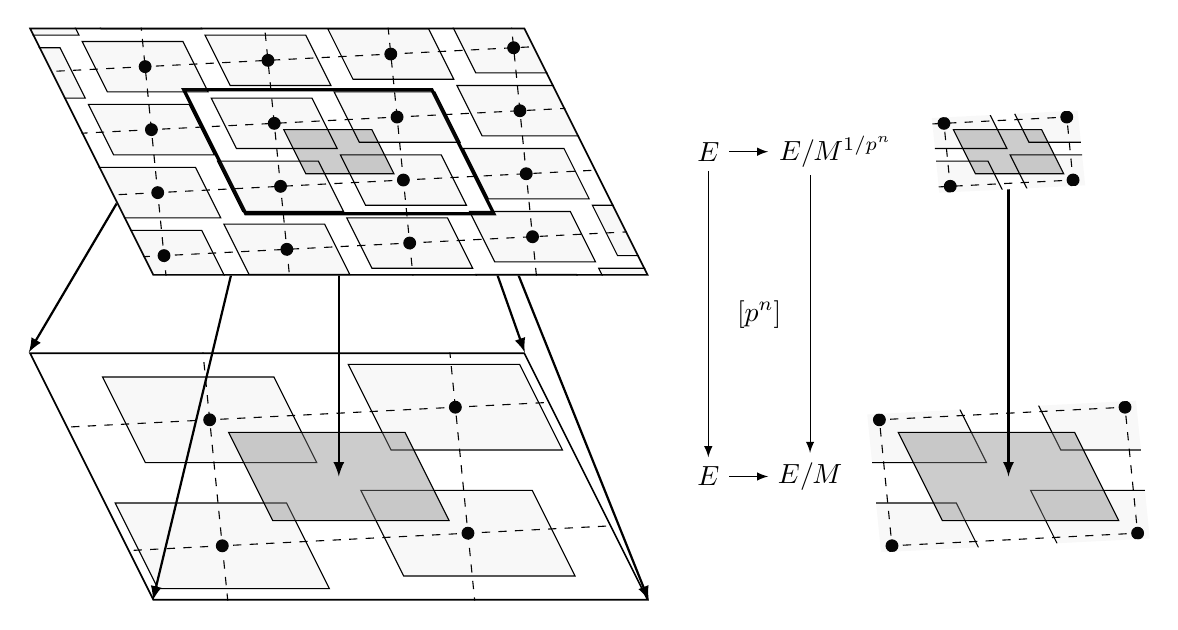
\begin{tikzpicture}


0.75

\def\shift{5.5*0.75}

\def\Aoffset{0.15}

%\pgfmathsetmacro\l{2.3*0.75}
%\pgfmathsetmacro\L{3.5*0.75}
%\def\s{0.4}
%\def\S{0.35}
%\def\Cl{4.55*0.75}


\pgfmathsetmacro\l{2*0.8}
\pgfmathsetmacro\L{4*0.8}
\def\s{0.34}
\def\S{0.35}
\def\Cl{4.2*0.75}

\pgfmathsetmacro\hoffset{\Cl/(4.55*0.75)*1.4}

\def\hshift{2.7*\Cl}

\def\A{1}
\def\B{0.1}
\def\C{0.2}
\def\D{1}
\pgfmathsetmacro\det{1/(\A*\D-\B*\C)}

\def\AA{1}
\def\CC{0}
\def\BB{-0.25}
\def\DD{0.5}

\begin{scope}

\pgftransformcm{\AA}{\CC}{\BB}{\DD}{\pgfpoint{0cm}{0cm}}

	\clip (-\Cl,-\Cl) rectangle (\Cl cm,\Cl cm); % Clips the picture...
	
	\filldraw[very thick,fill=white, fill opacity=1, draw=black] (-\Cl,-\Cl)
	rectangle (\Cl,\Cl);	
	
	\begin{scope}
	\pgftransformcm{\A}{\B}{\C}{\D}{\pgfpoint{0cm}{0cm}}
	% This is actually the transformation matrix entries that
	% gives the slanted unit vectors.
	\draw[dashed] (-2*\Cl,-2*\Cl) grid[step=\L cm,xshift=0.5*\L cm,yshift=0.5*\L cm] (3*\Cl,3*\Cl);
	% Draws a grid in the new coordinates.
	
	\foreach \x in {-4.5,-3.5,...,3.5}{% Two indices running over each
		\foreach \y in {-4.5,-3.5,...,3.5}{% node on the grid we have drawn 
			\node[draw,circle,inner sep=1.5pt,fill] at (\L*\x,\L*\y) {};
			% Places a dot at those points
		}
	}
	
	\end{scope}
	
	\foreach \x in {-4.5,-3.5,...,3.5}{% Two indices running over each
		\foreach \y in {-4.5,-3.5,...,3.5}{% node on the grid we have drawn 
			\filldraw[fill=gray, fill opacity=0.05, draw=black] (-\s*\L+\x*\L*\A+\y*\L*\C,-\s*\L+\x*\L*\B+\y*\L*\D)
			rectangle (\s*\L+\x*\L*\A+\y*\L*\C,\s*\L+\x*\L*\B+\y*\L*\D);
			
		}
	}
	
	\filldraw[fill=gray, fill opacity=0.4, draw=black] ({-\S*\L},{-\S*\L})
	rectangle ({\S*\L},{\S*\L});

\end{scope}




\begin{scope}[shift = {(\hshift,0)}]
\pgftransformcm{\AA}{\CC}{\BB}{\DD}{\pgfpoint{0cm}{0cm}}


\pgftransformcm{\A}{\B}{\C}{\D}{\pgfpoint{0cm}{0cm}}
\clip (-0.5*\L-\Aoffset,-0.5*\L-\Aoffset) rectangle (0.5*\L+\Aoffset,0.5*\L+\Aoffset); % Clips the picture...
\pgftransformcm{\det*\D}{-\det*\B}{-\det*\C}{\det*\A}{\pgfpoint{0cm}{0cm}}

\filldraw[very thick,fill=white, fill opacity=1, draw=black] (-\Cl,-\Cl)
rectangle (\Cl,\Cl);	

\begin{scope}
\pgftransformcm{\A}{\B}{\C}{\D}{\pgfpoint{0cm}{0cm}}
% This is actually the transformation matrix entries that
% gives the slanted unit vectors.
\draw[dashed] (-2*\Cl,-2*\Cl) grid[step=\L cm,xshift=0.5*\L cm,yshift=0.5*\L cm] (3*\Cl,3*\Cl);
% Draws a grid in the new coordinates.

\foreach \x in {-4.5,-3.5,...,3.5}{% Two indices running over each
	\foreach \y in {-4.5,-3.5,...,3.5}{% node on the grid we have drawn 
		\node[draw,circle,inner sep=1.5pt,fill] at (\L*\x,\L*\y) {};
		% Places a dot at those points
	}
}

\end{scope}

\foreach \x in {-4.5,-3.5,...,3.5}{% Two indices running over each
	\foreach \y in {-4.5,-3.5,...,3.5}{% node on the grid we have drawn 
		\filldraw[fill=gray, fill opacity=0.05, draw=black] (-\s*\L+\x*\L*\A+\y*\L*\C,-\s*\L+\x*\L*\B+\y*\L*\D)
		rectangle (\s*\L+\x*\L*\A+\y*\L*\C,\s*\L+\x*\L*\B+\y*\L*\D);
		
	}
}

\filldraw[fill=gray, fill opacity=0.4, draw=black] ({-\S*\L},{-\S*\L})
rectangle ({\S*\L},{\S*\L});

\pgftransformcm{\A}{\B}{\C}{\D}{\pgfpoint{0cm}{0cm}}{
	\clip (-\l,-\l) rectangle (\l,\l);}
\end{scope}





\pgfmathsetmacro\cl{\Cl*\l/\L} ;
\draw [thick,-latex] ({-\cl*(\AA+\BB)},{\shift-\cl*(\CC+\DD)}) -- ({-\Cl*(\AA+\BB)},{-\Cl*(\CC+\DD)});
\draw [thick,-latex] ({-\cl*\BB+\cl*\AA)},{\shift-\cl*(\CC+\DD)}) --({-\Cl*\BB+\Cl*\AA)},{\Cl*\CC-\Cl*\DD)});
\draw [thick,-latex] ({\cl*\BB+\cl*\AA)},{\shift+\cl*(\CC+\DD)}) --({\Cl*\BB+\Cl*\AA)},{\Cl*\CC+\Cl*\DD)});
\draw [thick,-latex] ({\cl*\BB-\cl*\AA)},{\shift+\cl*(\CC+\DD)}) --({\Cl*\BB-\Cl*\AA)},{-\Cl*\CC+\Cl*\DD)});


\draw [thick,-latex] (0,\shift) --(0,0);
\draw [thick,-latex] (\hshift,\shift) --(\hshift,0);

\def\A{1}
\def\B{0.1}
\def\C{0.2}
\def\D{1}





\begin{scope}[shift={(0,\shift)}]
\pgftransformcm{\AA}{\CC}{\BB}{\DD}{\pgfpoint{0cm}{0cm}}
\coordinate (Origin)   at (0,0);
\coordinate (XAxisMin) at (-2,0);
\coordinate (XAxisMax) at (3.7,0);
\coordinate (YAxisMin) at (0,-2);
\coordinate (YAxisMax) at (0,3.7);


\coordinate (offset)   at ({0.5*\l*(\A+\C)},{0.5*\l*(\B+\D)});


\clip (-\Cl,-\Cl) rectangle (\Cl cm,\Cl cm); % Clips the picture...

	
	\filldraw[very thick,fill=white, fill opacity=1, draw=black] (-\Cl,-\Cl) 
	rectangle (\Cl,\Cl);
	\filldraw[very thick,fill=white, fill opacity=0.1, draw=black] (-\Cl*\l/\L,-\Cl*\l/\L) 
	rectangle (\Cl*\l/\L,\Cl*\l/\L);



	\filldraw[fill=gray, fill opacity=0.4, draw=black] ({-\S*\l},{-\S*\l})
	rectangle ({\S*\l},{\S*\l});
	
	\def\s{0.4};
	\def\S{0.35};
	
	\begin{scope}
	\pgftransformcm{\A}{\B}{\C}{\D}{\pgfpoint{0cm}{0cm}}
	% This is actually the transformation matrix entries that
	% gives the slanted unit vectors.

	\draw[dashed] (-2*\Cl,-2*\Cl) grid[step=\l cm,xshift=0.5*\l cm,yshift=0.5*\l cm] (7,7);
	% Draws a grid in the new coordinates.
	
	\foreach \x in {-4.5,-3.5,...,3.5}{% Two indices running over each
		\foreach \y in {-4.5,-3.5,...,3.5}{% node on the grid we have drawn 
			\node[draw,circle,inner sep=1.5pt,fill] at (\l*\x,\l*\y) {};
			% Places a dot at those points
		}
	}
	
	
	%\node at (0.5*\l,0.5*\l) {$D$};
	\end{scope}
	
	
	\foreach \x in {-4.5,-3.5,...,3.5}{% Two indices running over each
		\foreach \y in {-4.5,-3.5,...,3.5}{% node on the grid we have drawn 
			\filldraw[fill=gray, fill opacity=0.05, draw=black] (-\s*\l+\x*\l*\A+\y*\l*\C,-\s*\l+\x*\l*\B+\y*\l*\D)
			rectangle (\s*\l+\x*\l*\A+\y*\l*\C,\s*\l+\x*\l*\B+\y*\l*\D);
			
		}
	}
	
	

\end{scope}






\begin{scope}[shift = {(\hshift,\shift)}]

\pgftransformcm{\AA}{\CC}{\BB}{\DD}{\pgfpoint{0cm}{0cm}}


\pgftransformcm{\A}{\B}{\C}{\D}{\pgfpoint{0cm}{0cm}}
\clip (-0.5*\l-\Aoffset,-0.5*\l-\Aoffset) rectangle (0.5*\l+\Aoffset,0.5*\l+\Aoffset);
\pgftransformcm{\det*\D}{-\det*\B}{-\det*\C}{\det*\A}{\pgfpoint{0cm}{0cm}}

	\filldraw[very thick,fill=white, fill opacity=1, draw=black] (-\Cl,-\Cl) 
	rectangle (\Cl,\Cl);
	\filldraw[very thick,fill=white, fill opacity=0.1, draw=black] (-\Cl*\l/\L,-\Cl*\l/\L) 
	rectangle (\Cl*\l/\L,\Cl*\l/\L);
	
	
	
	\filldraw[fill=gray, fill opacity=0.4, draw=black] ({-\S*\l},{-\S*\l})
	rectangle ({\S*\l},{\S*\l});
	
	\def\s{0.4};
	\def\S{0.35};
	
	\begin{scope}
	\pgftransformcm{\A}{\B}{\C}{\D}{\pgfpoint{0cm}{0cm}}
	% This is actually the transformation matrix entries that
	% gives the slanted unit vectors.
	
	\draw[dashed] (-2*\Cl,-2*\Cl) grid[step=\l cm,xshift=0.5*\l cm,yshift=0.5*\l cm] (7,7);
	% Draws a grid in the new coordinates.
	
	\foreach \x in {-4.5,-3.5,...,3.5}{% Two indices running over each
		\foreach \y in {-4.5,-3.5,...,3.5}{% node on the grid we have drawn 
			\node[draw,circle,inner sep=1.5pt,fill] at (\l*\x,\l*\y) {};
			% Places a dot at those points
		}
	}
	
	
	%\node at (0.5*\l,0.5*\l) {$D$};
	\end{scope}
	
	
	\foreach \x in {-4.5,-3.5,...,3.5}{% Two indices running over each
		\foreach \y in {-4.5,-3.5,...,3.5}{% node on the grid we have drawn 
			\filldraw[fill=gray, fill opacity=0.05, draw=black] (-\s*\l+\x*\l*\A+\y*\l*\C,-\s*\l+\x*\l*\B+\y*\l*\D)
			rectangle (\s*\l+\x*\l*\A+\y*\l*\C,\s*\l+\x*\l*\B+\y*\l*\D);
			
		}
	}
	


\end{scope}


\node(Q) at ({\Cl*1.9-\hoffset},\shift) {$E$};
\node(QQQ)  [label={[label distance=-1.05cm]0:$E/M^{1/p^n}$}] at ({\Cl*1.9},\shift) {\phantom{$E/M$}};

\node(P) at ({\Cl*1.9-\hoffset},0) {$E$};
\node(PPP) at (({\Cl*1.9},0) {$E/M$};

\node at (({\Cl*1.9-0.5*\hoffset},0.5*\shift) {$[p^n]$};

\draw[-latex] (Q.south) -- (P.north);
\draw[-latex] (QQQ.south) -- (PPP.north);
\draw[-latex] (Q.east) -- (QQQ.west);
\draw[-latex] (P.east) -- (PPP.west);

%\node(Q) at ({\Cl*2.1-\hoffset},\shift) {$E$};
%\node(QQ) at (({\Cl*2.1},\shift) {$E_j^{1/p^n}$};
%\node(QQQ)  [label={[label distance=-1.05cm]0:$E/M^{1/p^n}$}] at ({\Cl*2.1+\hoffset},\shift) {\phantom{$E/M$}};

%\node(P) at ({\Cl*2.1-\hoffset},0) {$E$};
%\node(PP) at (({\Cl*2.1},0) {$E_j$};
%\node(PPP) at (({\Cl*2.1+\hoffset},0) {$E/M$};

%\draw[-latex] (QQ.south) -- (PP.north);
%\draw[left hook-latex] (PP.west) -- (P.east);
%\draw[left hook-latex] (QQ.west) -- (Q.east);
%\draw[right hook-latex] (QQ.east) -- (QQQ.west);
%\draw[right hook-latex] (PP.east) -- (PPP.west);
%\draw[-latex] (Q.south) -- (P.north) node[midway,right] {$[p^n]$};
%\draw[-latex] (QQQ.south) -- (PPP.north) node[midway,left] {$[p^n]$};
	%

\end{tikzpicture}
\end{document}